	\documentclass[]{report}
\usepackage{tikz}
\newcommand{\inputtikz}[2]{%  
	\scalebox{#1}{\input{#2}}  
}
\usepackage[english]{babel}
\usepackage[utf8x]{inputenc}
\usepackage{amsmath}
\usepackage{graphicx}
%\usepackage[colorinlistoftodos]{todonotestfa}
\usepackage{listings}
\usepackage{color}
\usepackage{amsmath}
\usepackage{amsfonts}
\usepackage{mathtools}
\usepackage{graphicx}
\usepackage{caption}
\definecolor{dkgreen}{rgb}{0,0.6,0}
\definecolor{gray}{rgb}{0.5,0.5,0.5}
\definecolor{mauve}{rgb}{0.58,0,0.82}
%opening

\begin{document}
	
\begin{titlepage}
	
	\newcommand{\HRule}{\rule{\linewidth}{0.5mm}} 
	
	\center 
	
	\textsc{\LARGE Université de Technologie de Compiegne}\\[1.5cm]
	\textsc{\Large SY19}\\[0.5cm] 
	\textsc{\large Machine Learning}\\[0.5cm]
		
	\HRule \\[0.4cm]
	{ \huge \bfseries Second Assignment}\\[0.4cm] 
	\HRule \\[1.5cm]
		
	\begin{minipage}{0.4\textwidth}
		\begin{flushleft} \large
			Aladin \textsc{TALEB} 
		\end{flushleft}
	\end{minipage}
	~
	\begin{minipage}{0.4\textwidth}
		\begin{flushright} \large
			Zineb \textsc{SLAM} 
		\end{flushright}
	\end{minipage}\\[2cm]

	{\large \today}\\[2cm] 

	
\includegraphics[width=40mm]{Figures/utc.jpg}\\ % 

	\vfill
	
\end{titlepage}

\lstset{frame=tb,
	language=R,
	aboveskip=3mm,
	belowskip=3mm,
	showstringspaces=false,
	framexleftmargin=5mm,
	columns= fixed,
	numbers = left,
	basicstyle={\small\ttfamily},	
	numberstyle=\tiny\color{gray},
	keywordstyle=\color{blue},
	commentstyle=\color{dkgreen},
	stringstyle=\color{mauve},
	breaklines=true,
	breakatwhitespace=true,
	tabsize=3
}

	

\begin{abstract}
	

\end{abstract}


\tableofcontents



\section{Context}
This exercice aims to build the best classifier to recognize facial expressions based on a normalized photo of a given subject. The model will take advantage of a database of about 200 photos to learn how to classify the six different expressions : happiness, surprise, sadness, disgust, anger and fear.

\section{Dataset Description}
The very first step of our method consists in taking a look at the raw dataset. The dataset comprises 216 black and white photos of size 60 by 70, thus each case is described through 4200 features. Each feature represents a single pixel of the face, and the responses describe the facial expression. There are 6 kind of reponses : 1 to 6, each of which is described through 36 different photos. Below an example of each face expression:


\begin{center}
	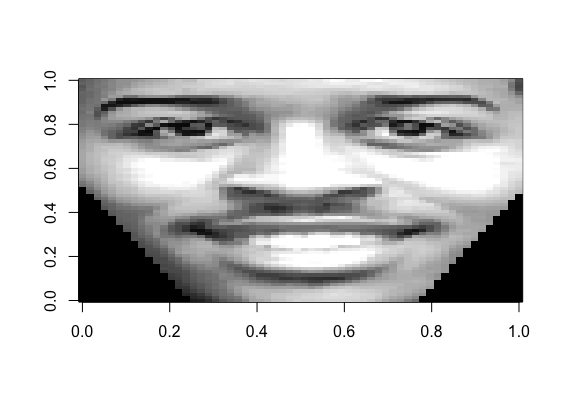
\includegraphics[width=0.6\linewidth]{Figures/happy_X32_y1.png}
	\captionof{figure}{y=1 Happy}
	\label{fig:y=1}
\end{center}

\begin{center}
	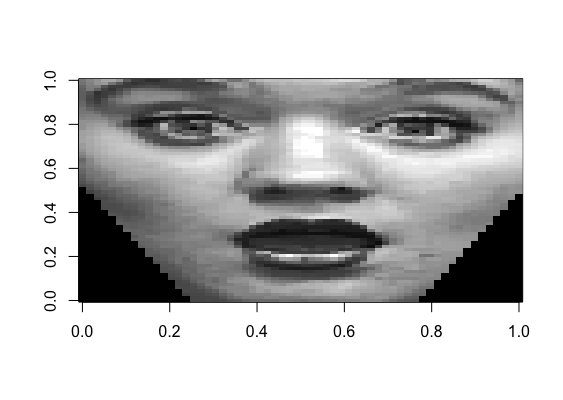
\includegraphics[width=0.6\linewidth]{Figures/shocked_X8_y2.png}
	\captionof{figure}{y=2 Shocked}
	\label{fig:y=2}
\end{center}

\begin{center}
	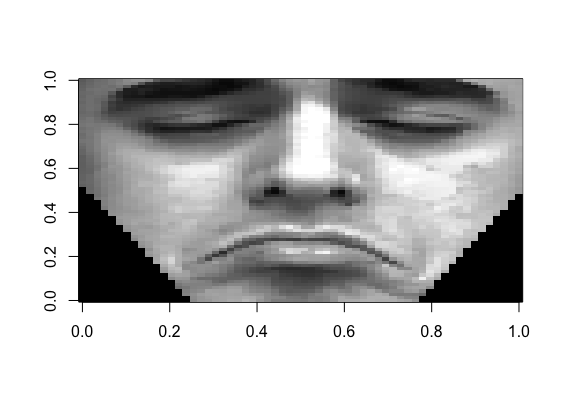
\includegraphics[width=0.6\linewidth]{Figures/cry_X132_y3.png}
	\captionof{figure}{y=3 Disapointed}
	\label{fig:y=3}
\end{center}

\begin{center}
	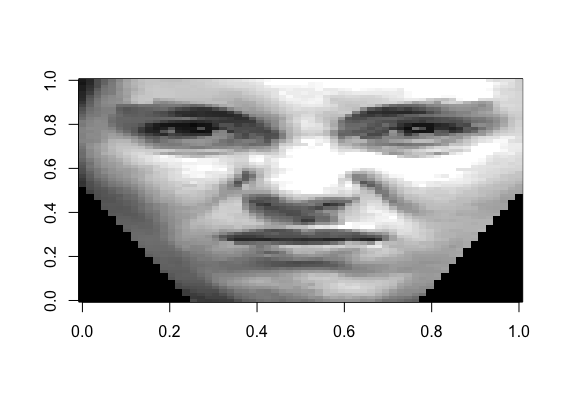
\includegraphics[width=0.6\linewidth]{Figures/mad_X54_y4.png}
	\captionof{figure}{y=4 Mad}
	\label{fig:}
\end{center}

\begin{center}
	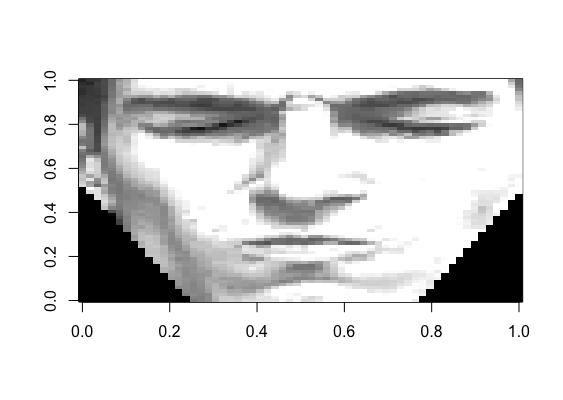
\includegraphics[width=0.6\linewidth]{Figures/angry_X10_y5.png}
	\captionof{figure}{y=5 Angry}
	\label{fig:y=6}
\end{center}

\begin{center}
	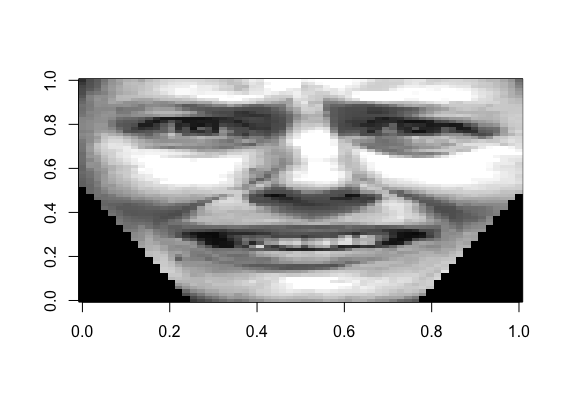
\includegraphics[width=0.6\linewidth]{Figures/sad_X204_y6.png}
	\captionof{figure}{y=6 Sad}
	\label{fig:y=6}
\end{center}

 It turns out that a non-negligible part of those features are null. Any null features may prevent the following classifiers to fit properly. The following code removes the null features from the dataset :
\begin{lstlisting}
X.clean= X[,colSums(X) != 0]
\end{lstlisting}
Each photo is now described through 3660 non-null features. Nevertheless, 3660 is still a very high number of features which prevents us from properly visualizing the dataset

\section{Measure to Compare Models}
Before building any model, we have to properly define the measures we will use later to compare their performance. In a classification problem, "accuracy" is often used. It is defined by :
$$
A = \frac{\text{Number of Good Predictions}}{\text{Number of Cases}}
$$

This is a very simple measure that may cause some issues when applied on classification problems that deal with skewed classes. For instance, let $A$ and $B$, two classes. $A$ contains 95\% of the dataset, while $B$ contains the remaining 5\%. Let $M$ a pretty bad classifier which classifies the whole dataset in class $A$. According to the definition stated above, this classifier has an accuracy of 95\%, which is excellent. In this case, more specific performance measures have to be applied.

However, our current classification problem does not deal with skewed class since all classes are equally-represented in the dataset. Therefore, we will be able to run this performance measure without any important issue. This measure will be applied on the test set in order not to include any bias.

\begin{lstlisting}
set.seed (1)
train = sample(1:n, round(2*n/3))

train.X= X.clean[train, ]
train.Y= as.matrix(y[train, ])

test.X= X.clean[-train, ]
test.Y= as.matrix(y[-train, ])

train_set= as.data.frame(cbind(train.Y, train.X))
test_set= as.data.frame(cbind(test.Y, test.X))
train_set= data.frame(train.X, y= as.factor(train.Y))
test_set= data.frame(test.X, y= as.factor(test.Y))
\end{lstlisting}

\pagebreak
\section{Classification}

\subsection{K Nearest Neighbors}
We can start our study with a very simple model like the KNN to have an idea about the Bayes error rate, which is the minimum achievable error rate. 

To perform a multi-classification in KNN we choose the k closest neighbor to each observation then each neighbor votes for a  class. At the end we pick the class that has the highest votes. 
First we perform a cross validation to pick the best k number of neighbors.

\subsubsection{Model Implementation}
To perform a CV on KNN we use the function \textbf{kknn.train} defined in the library \textbf{kknn}. As we do not have that much observation we can afford the computation of the Leave One Out.
\begin{lstlisting}
library("kknn")
model.kknn= train.kknn(y~., data= train_set, kmax = 30)
model.kknn.best.k = model.kknn$best.parameters$k
\end{lstlisting}
We find 28 to be the number of neighbors that minimizes the train error. Now we use this k on our knn model.

\begin{lstlisting}
library('FNN')
model.knn.pred= knn(train.X, test.X, train.Y ,k=model.kknn$best.parameters$k)
\end{lstlisting}

The KNN gives out the index of the 28 closest points to each observation. We then get the class of each of those neighbors using the function\textbf{ attr}. We count the cardinal of each class and pick the highest one to be the response of the observation.
\pagebreak

\begin{lstlisting}
n_test = nrow(test.X)
#Vector with prediction of the class of each test observation
knn_pred = matrix(, nrow=n_test , ncol=1) 

for(i in 1:n_test)
{

    #Class of each neighbor of the observation i
    iline = train_set$y[attr(model.knn.pred, 'nn.index')[i,]]
    # Count votes for each class
    count1 = length(which(iline[] == 1)) 
    count2 = length(which(iline[] == 2)) 
    count3 = length(which(iline[] == 3)) 
    count4 = length(which(iline[] == 4)) 
    count5 = length(which(iline[] == 5)) 
    count6 = length(which(iline[] == 6)) 
    #Vector of votes
    votes       = c(count1, count2, count3, count4, count5, count6)
    #I need to select the class with the highest number of neighbors
    max_vote = which.max(votes)
    knn_pred[i] = max_vote
}
\end{lstlisting}
The vector \textbf{knn\_pred} has the predicted response of each test observation. We construct the confusion matrix by comparing the true responses to the predicted ones. The values that are not in the diagonal are the miss-classified ones. We also compute the error.
\begin{lstlisting}
confusion_matrix_knn = table(predict=knn_pred , truth= test_set$y)
errors_knn = sum(knn_pred!=test_set$y)/length(test_set$y)
# 26.3% errors
\end{lstlisting}
\pagebreak
\subsubsection{Model Analysis}
The results of the KNN are shown below.
\begin{verbatim}
      truth
predict  1  2  3  4  5  6
      1 11  0  0  0  0  2
      2  0 15  0  0  0  1
      3  0  0  9  0  1  1
      4  1  1  1  8  2  3
      5  0  0  2  1  8  1
      6  2  0  0  0  0  2
0.2638889
\end{verbatim}
We notice that 19 observations out of 72 were miss-classified, we thus get 26\% of errors. Considering than the KNN is a very simple non parametric approach we can say that this is not a bad estimation. Therefore we will use more complex models in the next parts to minimize the test error. \textbf{But we know that 26\% will be our upper bound for the test error.}

\pagebreak

\subsection{LDA - Linear Discriminant Analysis}
The next classifier we are going to use is built using the Linear Discriminant Analysis (LDA) method, based on Bayes' Theorem. This simple and straight-forward model allows us to have a quick idea of the performance we can expect from more complex methods.  

\subsubsection{Method Implementation}
The function \texttt{lda} is available to fit the model onto a given dataset. It returns the group means that are the average of each predictor in each class. The coefficients of linear discriminants output are used to form the LDA decision rule. The prior probability is the percentage of the response for each class in the observation.

\begin{lstlisting}
library(MASS)
model.lda = lda(y ~ ., data = train_set)
summary(model.lda)
\end{lstlisting}

Due to the relatively high number of features, it takes a couple of seconds for the algorithm to fit the model.  Once the model is trained, we call the \texttt{predict} function to predict the responses of the test set : 

\begin{lstlisting}
model.lda.predicted = predict(model.lda, newdata = test_set)
perfMeasure(model.lda.predicted$class, test_set.y)
\end{lstlisting}

\begin{verbatim}
    class
pred  1  2  3  4  5  6
1 11  0  0  0  0  5
2  0  9  0  1  0  0
3  0  0  9  0  1  2
4  0  0  0 16  0  0
5  0  0  0  1  8  3
6  0  0  0  0  0  8

0.1756757
\end{verbatim}

\subsubsection{Data visualisation using FDA}
One of the biggest problems of high-dimensional spaces is the unability to easiliy plot it in order to study and to evaluate the boundaries that separate each class.

The FDA method allows us to greatly reduce the number of dimensions. More precisely, let $K$ the number of classes, FDA tries to describe the entire dataset using $K-1$ components. In our case, $K = 6$, therefore we can easily reduce the number of dimensions from 3660 down to only 5, which is way easier to plot.

\begin{lstlisting}
% APPLY FDA TRANSFORMATION
U = model.lda$scaling
Z = train_set.X %*% U

dim1 = 1
dim2 = 2

% PLOT EACH SAMPLE IN THE FDA SPACE
plot(Z[train_set.y==1,dim1],Z[train_set.y==1,dim2], xlim=range(Z[,dim1]),ylim=range(Z[,dim2]))
points(Z[train_set.y==2,dim1],Z[train_set.y==2,dim2],pch=2,col=2)
points(Z[train_set.y==3,dim1],Z[train_set.y==3,dim2],pch=3,col=3)
points(Z[train_set.y==4,dim1],Z[train_set.y==4,dim2],pch=4,col=4)
points(Z[train_set.y==5,dim1],Z[train_set.y==5,dim2],pch=5,col=5)
points(Z[train_set.y==6,dim1],Z[train_set.y==6,dim2],pch=6,col=6)
\end{lstlisting}

\begin{center}
	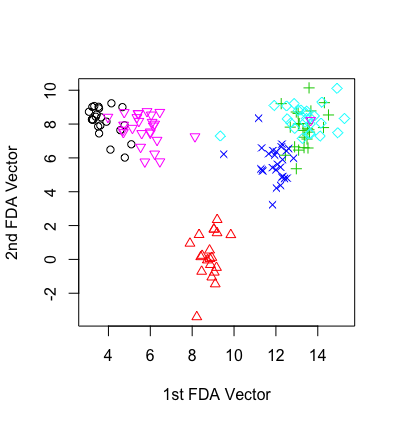
\includegraphics[width=0.6\linewidth]{Figures/plot_fda_1_2.png}
	\captionof{figure}{Plot of the train set using a projection onto the first two components of the FDA space.}
	\label{fig:plot_fda_1_2}
\end{center}

\subsubsection{Dimension Reduction with PCA}
3660 is a quite high-number of features that slows down both fitting and prediction algorithms, and which may prevent the model from fitting properly. More specifically, the number of dimensions of this dataset is way higher than the number of samples, which means that the model may not be able to capture all relationships between the inputs and the response. One way of improving the performance of the algorithm, both in terms of accuracy and speed, is to decrease the number of inputs.

The FDA methods described previously is a very powerful dimension reduction technique that consists in changing the space using a linear transformation. However, LDA's accuracy score doesn't depends on space transformation, thus coupling FDA with LDA does not make any change.

Another way of reducing the number of features is using a Principal Component Analysis method. Such method aims to find the set of vectors, called principal components, that best describe the features variance. We can then select the best subset of principal components, which is the set of features that yields to the highest performance.

\begin{lstlisting}
fit_lda_pca = function() {
	model.lda.pca = lda(y ~ ., data = train_set.pca)
	model.lda.pca.predicted = predict(model.lda.pca, newdata = test_set.pca)
	p = perfMeasure(model.lda.pca.predicted$class, test_set.pca$y)
	return(p)
}

\end{lstlisting}

The function \texttt{prcomp} is available to compute the set of principal components using linear transformations. The same sequence of linear transformations should be applied on the test set as well, using the function \texttt{predict} : 
\begin{lstlisting}
pca = prcomp(train_set.X, center = TRUE, scale = TRUE)
nb_comp = 10 #Arbitrary Number

train_set.pca.X = as.data.frame(pca$x[,1:nb_comp])
train_set.pca = data.frame(train_set.pca.X)
train_set.pca["y"] = train_set.y

test_set.pca.X = predict(pca, newdata = test_set.X)[,1:nb_comp]
test_set.pca = data.frame(test_set.pca.X)
test_set.pca["y"] = test_set.y

fit_lda_pca()
\end{lstlisting}

The performance now mostly relies on the number of principal components used to describe the dataset. This parameter should be determined using a cross-validation technique as not to introduce any biais. Since fitting a LDA model does not take much time, we decided to use a 10-fold cross validaiton method between : 

\begin{lstlisting}
nb_folds = 10
accs = matrix(0, 100, 1)
accs[1] = Inf
for (M in 2:100) {
	printf("Nb PCA %d", M)
	a.train_set.pca.X = as.data.frame(pca$x[,1:M])
	a.train_set.pca = data.frame(a.train_set.pca.X)
	a.train_set.pca["y"] = train_set.y
	
	a.test_set.pca.X = predict(pca, newdata = test_set.X)[,1:M]
	a.test_set.pca = data.frame(a.test_set.pca.X)
	a.test_set.pca["y"] = test_set.y
	
	folds = createFolds(a.train_set.pca$y, k = nb_folds)
	
	acc = 0;
	for (k in 1:nb_folds) {
		validation_indexes = folds[[k]]
		train_set.pca.X = a.train_set.pca.X[-validation_indexes,]
		train_set.pca = a.train_set.pca[-validation_indexes,]
		
		test_set.pca.X = a.train_set.pca.X[validation_indexes,]
		test_set.pca = a.train_set.pca[validation_indexes,]
		
		acc = acc + fit_lda_pca()
	}
	
	acc = acc / nb_folds
	accs[M] = acc
}
min(accs)
which.min(accs)
\end{lstlisting}

We ran this algorithm many times and we found different results depending on the cross-validation split : 

\begin{center}
	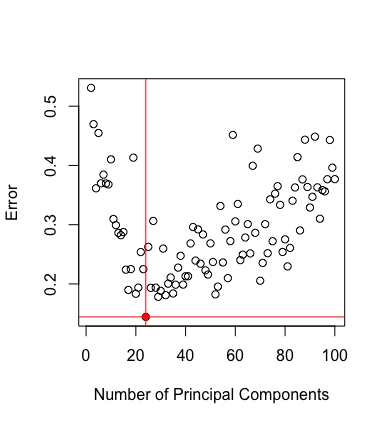
\includegraphics[width=0.6\linewidth]{Figures/lda_pca_cv.png}
	\captionof{figure}{10 fold cross validation to find the best number of components to use for LDA.}
	\label{fig:lda_pca_cv}
\end{center}

\begin{center}
	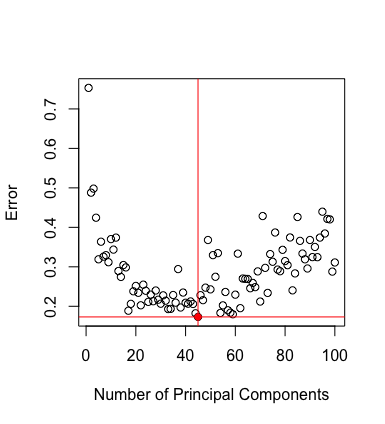
\includegraphics[width=0.6\linewidth]{Figures/lda_pca_cv_2.png}
	\captionof{figure}{Another 10 fold cross validation to find the best number of components to use for LDA.}
	\label{fig:lda_pca_cv_2}
\end{center}

It turns out that the 45 components yields to the lowest cross-validation error rate of about 17\%. We can now apply this model on the test set : the error-rate can be as low as 12\%.

\pagebreak

\subsection{Neural Networks}

Neural Networks are a set of methods based on a collection of computation units called artificial neurons, each of which is basically capable of extracting a new features based on a linear combination of its inputs. The training algorithms then consists in tweaking each neuron so that it extracts the feature that minimize the error-rate of the whole network.

These classifiers are very powerful, but this power comes to a price of : 
\begin{itemize}
	\item a very long training time
	\item a non-convex error function to optimize, which means the optimization algorithm may reach a local optima
	\item a high number of parameters one should tweak in order to come up with the best network for a given dataset
\end{itemize}

To simplify our analysis, we will only deal with single hidden layer perceptrons. In R, the library \texttt{nnet} is available to build simple neural network classifiers and regression models : 
\begin{lstlisting}
library(nnet)

train_set$y = factor(train_set$y)
test_set$y = factor(test_set$y)

model.nnet = nnet(y ~ ., data=train_set, size=5, MaxNWts = 20000)
model.nnet.predicted = predict(model.nnet, test_set, type="class")
perfMeasure(model.nnet.predicted, test_set$y)
\end{lstlisting}

\subsubsection{Dimension Issue}

However, in our case, the number of features is way too high for a casual computer. Indeed, a single layer perceptron is described through $W$ parameters which represent the neurons' weights : 

$$
	W = M(P+1) + K(M+1)
$$

with $M$ the number of neurons, $P$ the number of features and $K$ the number of classes. In our case, $W = 3667M + 1$.
 therefore, the only parameter we have to tweak is the number of neurons contained in the hidden layer. This number should be determined using a cross-validation technique. However, even though $W$ doesn't grow exponentionally, it increases too fast for the fitting algorithm to perform in a timely manner. 
 
 We were able to fit a neural network with only 2 and 5 hidden neurons, it took respectively less than a minute and about 10 minutes to train the model. They both yield to miserable error rates of 85\% and 50\%. The main problem here is the ridiculously low number of neurons, a good rule of thumb being choosing $M$ between $K$ and $P$.
 
The main way to carry the analysis further would be to first apply a dimension reduction algorithm on the inputs.

\subsubsection{Dimension Reduction}
One such reduction algorithm is the FDA that we have already described previously. We now only have to cope with 5 different inputs, which is way easier for the optimization algorithm to work with. 

A 10-fold cross-validation algorithm can be performed in a timely manner. $M = 95$ yields to a very low error-rate of 5\% on the validaiton set, but a quite high error-rate of 27\% on the test set. This difference in the error-rate comes from the fact that a single hidden layer tend to overfit with a high number of neurons.

\begin{center}
	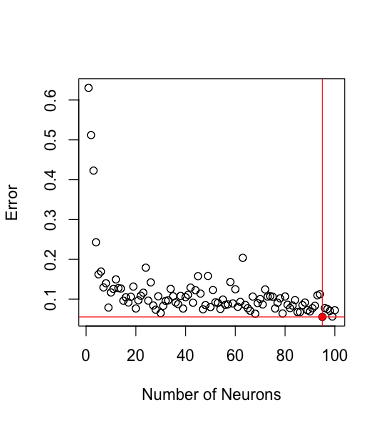
\includegraphics[width=0.6\linewidth]{Figures/nnet_fda_cv.png}
	\captionof{figure}{10 fold cross validation to find the best number of neurons.}
	\label{fig:nnet_fda_cv}
\end{center}

We could also take advantage of a Principal Component Analysis method to decrease the dimension. However, this would mean performing a nested cross-validation method in order to find the best number of components that goes with the best number of neurons.

\subsubsection{Regularization}
 It is possible to prevent the neural network from overfitting by using a regularization technique that basically constraints each neuron's weights using a parameter $\lambda$. The main idea is now to use a high number of neurons, before finding the best regularization parameter  $\lambda$ by cross-validation.
 
 We first apply this method on the dataset whose dimensions have been reduced using the FDA technique. Using $M = 50$, a fairly high number compared to the number of inputs and outputs, the best $\lambda$ seems to be 2, which yields to an error-rate ranged from 16\% to 20\% depending on the optimization results.
 
 \begin{center}
 	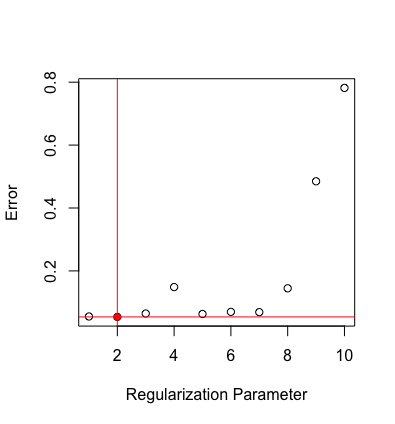
\includegraphics[width=0.6\linewidth]{Figures/nnet_fda_reg_cv.png}
 	\captionof{figure}{10 fold cross validation to find the best regularization term $\lambda$}
 	\label{fig:nnet_fda_reg_cv}
 \end{center}
\pagebreak

\subsection{Decision Trees}
 In this section, we will discuss a set of machine learning methods called decision trees. A decision tree is a very intuitive way to build a classifier (or a regression model) that aims to split the space into smaller pieces, a simple condition is then defined on a single parameter to guide the decision throughout the decision space. A classification tree is often used when an understable and interpretable classifier is needed. However, in our case, we do not need such property.
 
 A single tree can be grown using the function \texttt(tree) available in the library of the same name : 
 \begin{lstlisting}
 library(tree)
 
 model.tree = tree(as.factor(y) ~ ., train_set) 
 model.tree.predicted = predict(model.tree, test_set, type="class")
 \end{lstlisting}
 
  \begin{center}
 	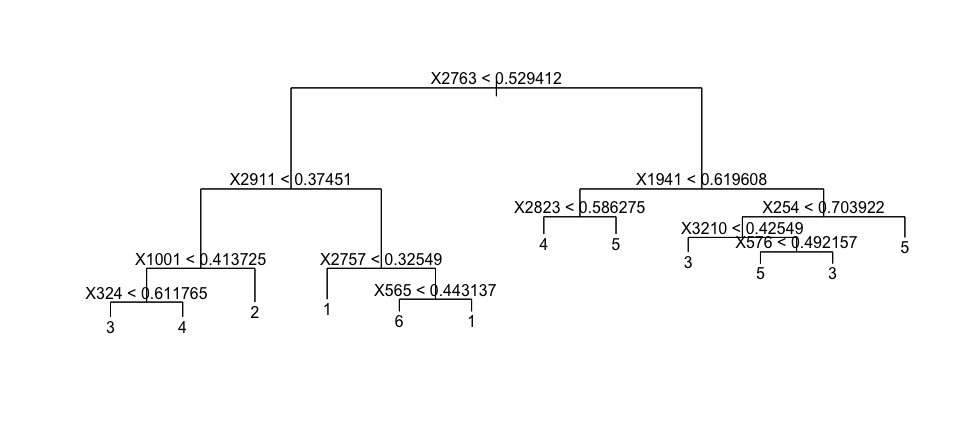
\includegraphics[width=0.6\linewidth]{Figures/tree_full.png}
 	\captionof{figure}{Decision Tree}
 	\label{fig:tree_full}
 \end{center}
 
 The grown tree has only 12 terminal nodes. The error-rate on the train set is less than 10\%, however the error-rate on the test set is over 40\%, which means this tree tends to overfit the train set. We could slightly improve the performance of the tree by pruning it using a cross validation method, but this would not make much sense for a 3660-dimension space made of very low-level features : how could a handful of conditions on pixel values could be enough to determine the correct emotion in most cases ?
 
 That is why we can once again reduce the number of dimensions using FDA. The tree has a 7 terminal nodes, a 10 fold cross-validation algorithm confirms that there is no need for pruning this tree. This decision tree yields to an error-rate of about 20\%.
 
   \begin{center}
 	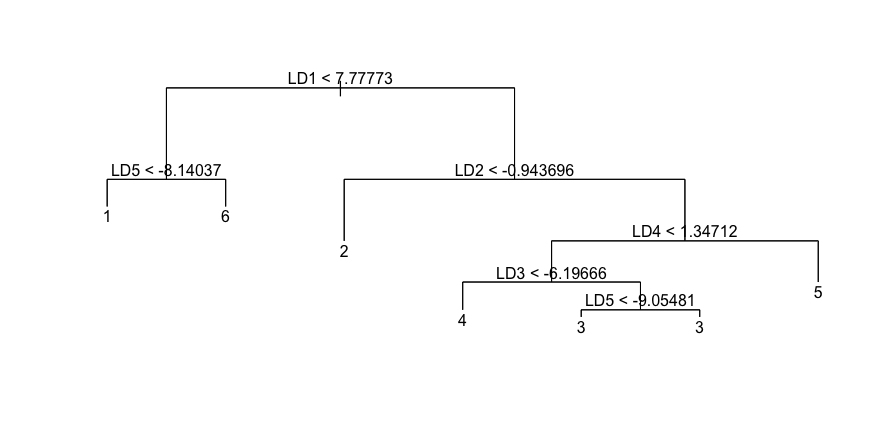
\includegraphics[width=0.6\linewidth]{Figures/tree_fda.png}
 	\captionof{figure}{Decision Tree}
 	\label{fig:tree_fda}
 \end{center}
 
    \begin{center}
 	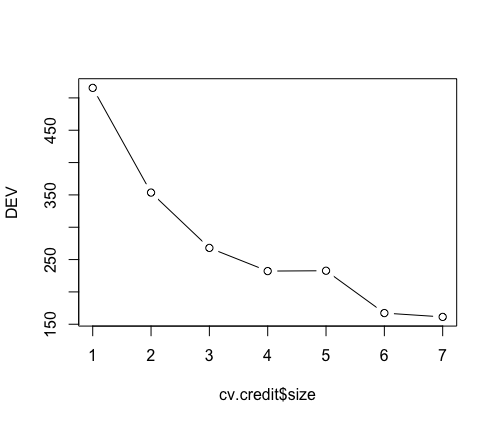
\includegraphics[width=0.6\linewidth]{Figures/tree_fda_cv.png}
 	\captionof{figure}{Best size}
 	\label{fig:tree_fda_cv}
 \end{center}
 
 It is possible to improve the accuracy of such methods by combining multiple decision trees, the main tradeoff being the unability to interpret the final classifier. This technique consists in building $B$ classification trees using slightly different datasets, getting the response related to an input can be done by having each tree vote for a single class.
 
\begin{lstlisting}
library(randomForest))

model.random_forest =randomForest(as.factor(y) ~ ., data=train_set)
model.random_forest.predicted = predict(model.random_forest,newdata=test_set,type='response')
\end{lstlisting}

We obtain an error-rate of 27\% with the raw dataset, which is better than using a single tree. However, the error-rate on the FDA dataset is still 20\%.
 
\pagebreak
\subsection{Support Vector Machines}
In this part we discuss another approach of classification : The Support Vector Machine with the kernel option. Our data set has a very large number of features compared to observations \textbf{(p>>n)}. This means that likely we could use a linear kernel. In Other words we want to compare SVMs with a linear kernel.
\subsubsection{Model Implementation}
The \textbf{e1071} library includes the \textbf{tune()} function, to perform Cross-Validation (by default, it performs 10-fold cross-validation) to determine the best tuning parameter.
\begin{lstlisting}
library('e1071')
model.tune = tune(svm, y~., data= train_set, kernel= "linear", ranges= list(c(0.01, 0.1, 1, 10), gamma= c(0.1, 1, 10)))
summary(model.tune)
\end{lstlisting}
The results of the 10 fold Cross validation are:
\begin{verbatim}
Parameter tuning of ‘svm’:
- sampling method: 10-fold cross validation 
- best parameters:
 Var1 gamma
 0.01   0.1
\end{verbatim}
We see the cost=0.01 results in the lowest cross-validation error rate as well as gamma=0.1.\\
The \textbf{tune()} function stores the best model that can be accessed as follows: \textbf{model.tune\$best.parameters} We can now perform the SVM model with those best tuning parameters.
The argument \textbf{scale=TRUE} tells the \textbf{svm()} function to scale each feature to have mean zero or standard deviation one;\textbf{ Should we scale (???)}. If the response has more than two levels, then the svm() function will perform multi-classification using the One-Versus-One approach.
\begin{lstlisting}
model.svm= svm(y~., data= train_set, kernel= 'linear', gamma= model.tune$best.parameters$gamma, cost= model.tune$best.parameters$Var1)
summary(model.svm)
\end{lstlisting}
The results are displayed below:
\begin{verbatim}
Parameters:
   SVM-Type:  C-classification 
 SVM-Kernel:  linear 
       cost:  0.01 
      gamma:  0.1 
Number of Support Vectors:  124
 ( 14 22 22 20 21 25 )
Number of Classes:  6 
Levels: 
 1 2 3 4 5 6
\end{verbatim}
We see that the function identified 6 classes. This tells us, for instance, that a linear kernel was used with cost=0.01 , and that there were 124 support vectors, 14 in class 1, 22 in class 2, 22 in class 3, 20 in class 4, 21 in class 5 and 25 in class 6. 
We can now plot the support vector classifier obtained:
\begin{lstlisting}
plot(x= model.svm, data= svm.train, formula= X1~X2)
\end{lstlisting}
\begin{center}
	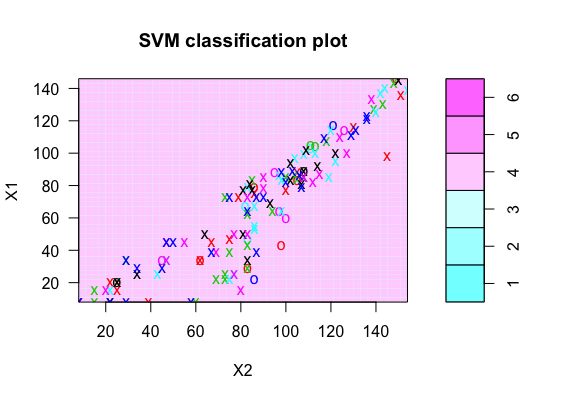
\includegraphics[width=0.8\linewidth]{Figures/svm_train_plot.png}
	\captionof{figure}{SVM on train set observations}
	\label{SVM on train set}
\end{center}

We Note that here the second feature is plotted on the x-axis and the first feature is plotted on the y-axis, 
The region that is assigned to each class is shown on the right (light blue for 1 to dark purple for 6). The decision boundary between the two classes is linear 
(because we used the argument kernel="linear"). 
\\We then computer the errors and the confusion matrix.
\pagebreak
\begin{lstlisting}
confusion_matrix_svm.train = table(model.svm$fitted, train_set$y)
errors_svm.train = sum(model.svm$fitted != train_set$y)/length(train_set$y)
\end{lstlisting}
\begin{verbatim}
   1  2  3  4  5  6
  1 22  0  0  0  0  0
  2  0 20  0  0  0  0
  3  0  0 24  0  0  0
  4  0  0  0 27  0  0
  5  0  0  0  0 25  0
  6  0  0  0  0  0 26
0
\end{verbatim}
Our train error is null, no observation were miss-classified while training the model. This is not really surprising as we have only 144 observations but 3360 variables. Since p>>n it was easy for the model to define a hyperplane that fully separates the classes. \\

However we are more interested in the support vector classifier’s performance on the test observations. We call the predict function that takes the SVM model as parameter.
\begin{lstlisting}
yhat= predict(model.svm, newdata= test_set)
confusion_matrix_svm.test= table(yhat, test_set$y)
errors_svm.test = sum(yhat!=test_set$y)/length(test_set$y)
plot(x= model.svm, data= test_set, formula= X1~X2)
\end{lstlisting}
\begin{verbatim}
 yhat  1  2  3  4  5  6
   1 12  0  0  0  0  1
   2  0 13  0  0  0  0
   3  0  0 10  0  1  2
   4  0  1  0  9  3  0
   5  0  2  2  0  7  0
   6  2  0  0  0  0  7
 0.1944444
\end{verbatim}

\begin{center}
	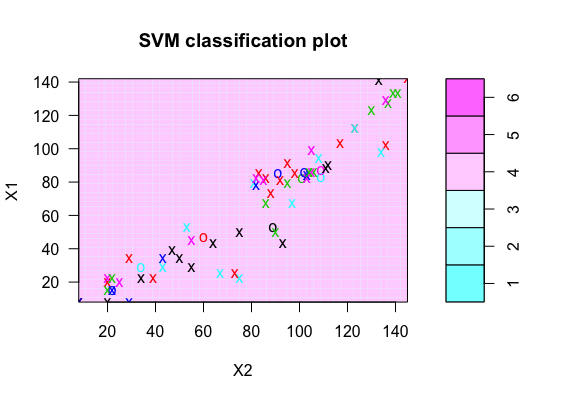
\includegraphics[width=0.8\linewidth]{Figures/svm_test_plot.png}
	\captionof{figure}{SVM on test set observations}
	\label{SVM on test set}
\end{center}
\subsubsection{Model Analysis}
Hence, with cost=0.1, 20 observations were miss-classified, our test error is equal to 19,4\%.


\pagebreak
\section{Conclusion}
\begin{center}
\begin{tabular}{l c}
\textbf{Model} & \textbf{Percentage of error} \\
KNN & 26.8\% \\
LDA & 17\% \\
LDA + PCA & 12/13\% \\
NNET + FDA & 27\% \\
NNET + FDA + Regularization & 16\% \\
Random Forest + FDA & 20\% \\
SVM & 19.4\%
\end{tabular}
\end{center}
\end{document}
